\chapter{Classifier}  \label{sec:classifier}

k-nearest neighborhood

Naive bayesian

SGD classifier + loss function + regularization term% http://scikit-learn.org/stable/modules/sgd.html#mathematical-formulation

\section{Decision tree and random forest}

Decision tree is a simple learning method that can be used for classification or regression. The implementation used of decision tree is based on the CART (Classification and Regression Tree) algorithm.

A decision tree is recursively partitioning the space in a left $P_{left}$ and right $P_{right}$ partitions such that the samples with the same labels are grouped together, i.e. the generated sets with the smallest impurity.

It continues to split until the impurity can't be reduced or some pre-set stopping rules are met. Alternatively, the data are split as much as possible and then the tree is later pruned.

Since the set of splitting rules used to segment the predictor space can be summarized in a tree, these types of approaches are known as decision tree methods. The figure  \ref{fig:decision_tree_simple_example} illustrate a toy example of decision tree.

\begin{figure}[h]
    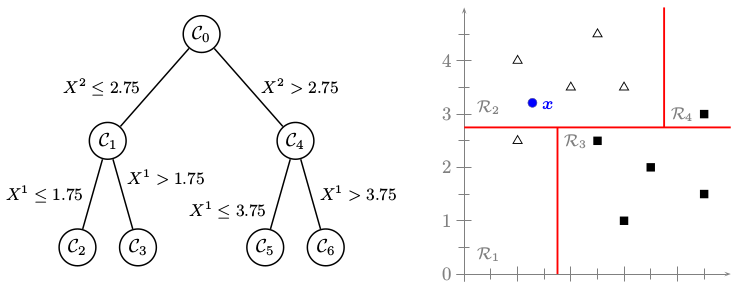
\includegraphics[scale=0.5]{img/decision_tree_simple_example}
    \caption[Decision tree of for ten elements belonging to two classes]{Decision tree of depth two for ten elements $(X^1, X^2)$ belonging to the black square and white triangle classes}
    \label{fig:decision_tree_simple_example}
\end{figure}

The most used impurity measure's functions are:
\begin{itemize}
    \item \textbf{Gini}: $$H(X_m) = \sum_k p_{mk} (1 - p_{mk})$$
    \item \textbf{Cross-entropy}: $$ H(X_m) = - \sum_k p_{mk} \log(p_{mk}) $$
\end{itemize}

To avoid overfitting, keep the decision tree as simple as possible.

\textbf{Random forest} or Decision forest is build from a number of decision trees. The prediction of the ensemble is given as the averaged prediction of the individual classifiers. Each tree is trained on a random subsets of the training data.

When building these decision trees, each time a split in a tree is considered, a random sample of
$m$ predictors is chosen as split candidates from the full set of $n$ features. A typical value of $m$ is $m \approx \sqrt{n}$.

\section{Support Vector Machine}

 (binary case) + kernel trick + multi-class (one-versus-one or one-versus-all)

\textbf{Support Vector Machine} \textit{SVM} is a method used for classification and regression.

\subsection{Linear SVM}
\subsubsection{Hard margin}

A support vector machine constructs a hyper-plane or set of hyper-planes in a high or infinite dimensional space. Intuitively, a good separation is achieved by the hyper-plane that has the largest distance to the nearest training data points of any class (so-called functional margin), since in general the larger the margin the lower the generalization error of the classifier.

For a 2 classes (value represented as $-1$ and $1$), the hyperplane must verify:
\begin{equation}\label{eq:svm_1}
    \vec{x_i} \cdot \vec{w} + b \geq + 1 \text{ for } y_i = + 1
\end{equation}
\begin{equation}\label{eq:svm_2}
    \vec{x_i} \cdot \vec{w} + b \leq -1 \text{ for } y_i = - 1
\end{equation}
where $\vec{w}$ is the normal to the hyperplane

Combining equation \ref{eq:svm_1} and \ref{eq:svm_2}, we obtain:
$$ \forall i \in {0, \ldots, n}, ~~ y_i (\vec{x_i} \cdot \vec{w} + b) - 1 \geq 0$$
where $y_i = f(\vec{x_i}) = {-1, 1}$

Gemetrically, the distance between the two hyperplane from \ref{eq:svm_1} and \ref{eq:svm_2} is $\frac{2}{\vec{w}}$ (equal width to each side).

Thus, to obtain the hyperplane with the highest margin, we want to maximize:
$$ \underset {\vec{w}, \vec{b}}{\argmax} \frac{2}{\lVert \vec{w} \rVert^2} $$
which is equivalent to minimize:
$$ \underset {\vec{w}, \vec{b}}{\argmin} \frac{1}{2} \lVert \vec{w} \rVert^2 $$

Thus, we obtain a constrained optimization problem.

\subsubsection{Soft Margin}

For the case of non-separable training sets, we introduce a penality parameter $C$, $C \leq 0$ and obtain:
$$
\underset {\vec{w}, \vec{b} \zeta}{\argmin} \frac{1}{2} \lVert \vec{w} \rVert^2 + C \sum_{i = 1}^{n} \zeta_i
\text{ subject to } y_i (\vec{x_i} \cdot \vec{w} + b) \geq 1 - \zeta_i, \zeta_i \geq 0, \forall i \in [1, \ldots, n]
$$

The decision function for new example is:
$$
f(\vec{x}) = \sign (\sum_{s_i \in \text{ support vectors}} w_i \vec{s_i} \cdot \vec{x} + b)
$$
where the support vectors selected sub-set of the training  examples that define the boundary of the hyperplane separation and hence the classification boundary.

To generalize SVM to the case of multi-class, multiple approaches are possible:
\begin{itemize}
    \item \enquote{one-versus-one}: train a separate classifier for each different pair of labels. This leads to $\frac{N (N - 1)}{2}$ classifiers
    \item \enquote{one-versus-all}: train a single classifier per class, with the samples of that class as positive samples and all other samples as negatives
\end{itemize}

\subsection{Non-linear SVM and kernel trick}

The idea of the kernel trick is to transform the initial space to a higher dimensional space where a hyperplane can separate this data.
Kernel trick: use kernel function to implicitly transform datasets to a higher-dimensional using no extra memory, and with a minimal effect on computation time: realise just a dot product.

To use the linear SVM for non-linear data: project the data in a new feature H space thanks to an application and then reserch for maximum margin hyperplan in H
to make sure that the new problem has a unique solution, 
must satisfy the Mercer's condition or simply it must be a positiv-definit matrix

\begin{itemize}
    \item \textbf{Linear} : $k(x, y) = \langle \vec{x} , \vec{y} \rangle + C = x^T y + C$
    \item \textbf{Polynomial}: $k(x, y) = (\gamma \cdot \langle \vec{x} , \vec{y} \rangle + C)^d = (\gamma \times x^T y + C)^d$
    \item \textbf{Radial Basis Function (RBF)}: $k(x, y) = \exp \left( - \gamma \lVert x - y \rVert ^2 \right)$
    \item \textbf{Chi-Square}: $\displaystyle k(x, y) = 1 - \sum_{i=1}^n \frac{(x_i-y_i)^2}{\frac{1}{2} (x_i+y_i)}$
    
    A modified version presented in \cite{Vedaldi2010} of this kernel is the \textbf{Additive Chi-Square} kernel :
    $\displaystyle k(x, y) = \sum_{i=1}^n \frac{2 (x_i - y_i)}{x_i + y_i} $
\end{itemize}

The adjustable parameters of these kernels are $d$, $\gamma$, $C$ and must be choosen according to the problem.

For food classification, the chi square kernel is the most used kernel as it is often combined with histograms. !!CITE!!

\section{Convolutional neural network}

A \textbf{Convolutional Neural Netwrok} \textit{CNN} is a variant of a Neural Network, mainly used for machine learning on pictures. It is inspired by the neural system composed of different layers (made up of multiple neurons) and communication shemes.

Each neuron receives some inputs, performs a dot product and optionally follows it with a non-linearity function. The whole network still expresses a single differentiable score function (linear or not): from the raw image pixels (the input layer) to class scores (output layer). Hidden layers separates these two layers, as described in \ref{fig:nn_3_layer}.

A CNN (and more generally a NN) is trained by backpropagation, applying gradient descent that will update the weights.

It is a powerful, adaptive and noise resilient pattern recognition. The training phase is rather slow but querying it with an unseen example is fairly fast.

\begin{figure}[h]
    \centering
    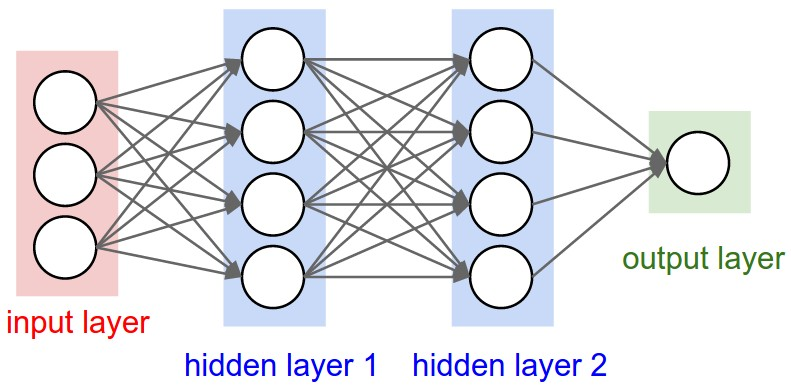
\includegraphics[scale=0.4]{img/nn_3_layers.jpeg}
    \caption{A regular 3-layer neural network}
    \label{fig:nn_3_layer}
\end{figure}

\begin{figure}[h]
    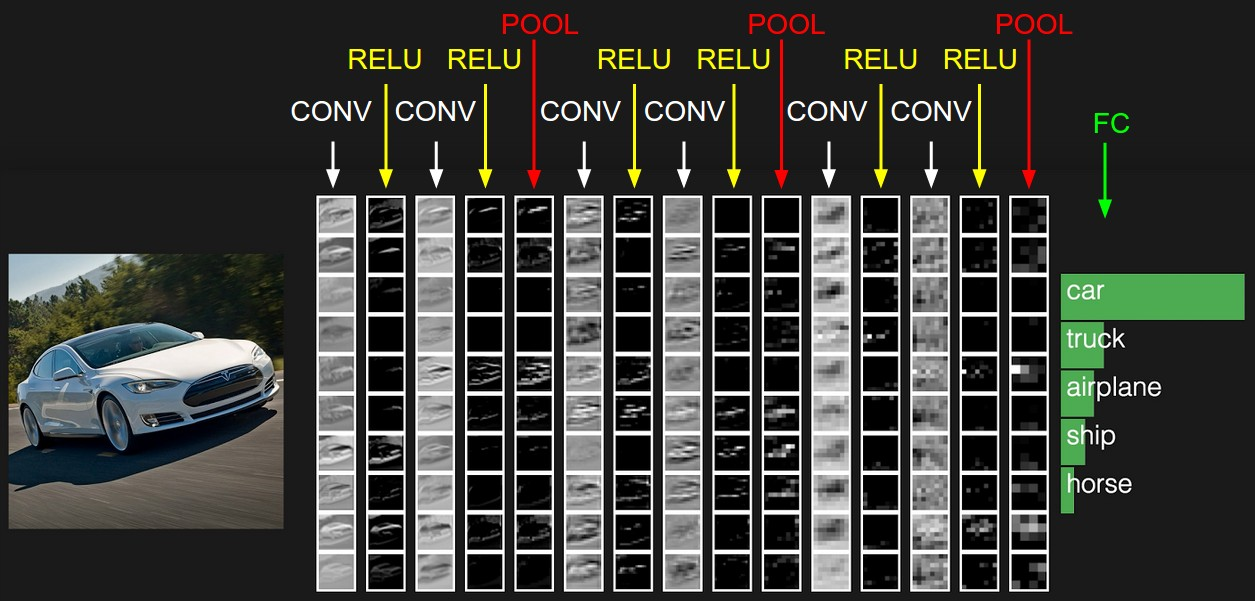
\includegraphics[scale=0.35]{img/cnn_simple_example.jpeg}
    \caption[Example of a 16-layer deep convolutional neural network]{Example of a 16-layer deep convolutional neural network. The input layer is a whole picture, the output layer is the probability for each possible class. It used a succession of Convolutional, ReLU, Pooling layer with a final Fully connected one.}
    \label{fig:cnn_simple_example}
\end{figure}

The figure \ref{fig:cnn_simple_example} is a simple CNN based on the VGG-NET structure. It is composed of the 4 most popular layers that can be found in a CNN:
\begin{itemize}
    \item \textbf{Convolutional} : layer fiving the name for this type of neural network. It convolves the input image with a set of learnable filters, each producing one feature map in the output image, i.e. it computes a dot product on a neighborhhod of pixels:
    
    $$ y_{i, j} = b + \sum_{l=0}^{n - 1} \sum_{m=0}^{n - 1}  w_{l,m} x_{j+l, k+m} $$
    with:
    \begin{itemize}
        \item $x_{i,j}$ the input activation at position $(x, y)$
        \item $w_{l, m}$ the weights of the neuron
        \item $n \times n$ is the size of the layer
        \item $b$ is the bias value
        \item $y_{i, j}$ the output values of the $j$, $k$th neuron
    \end{itemize}
    
    \item \textbf{Activation layer}: element wise operation.
    
    Example of function: the \textbf{Rectified Linear Unit} \textit{ReLU} defines as:
    $$ f(x) = max(0, x)$$
   
    \item \textbf{Pooling} or subsampling layer: down sampling of the input activation size. It reduces the number of values between the input and the output values of this layer to avoid overfitting the data and reduce the computation time of the neural network.
    
    The most common downsampling operation is max, giving rise to \textbf{max pooling}, here shown with a stride of 2 in figure \ref{fig:max_pooling}.
    
    \begin{figure}[h]
        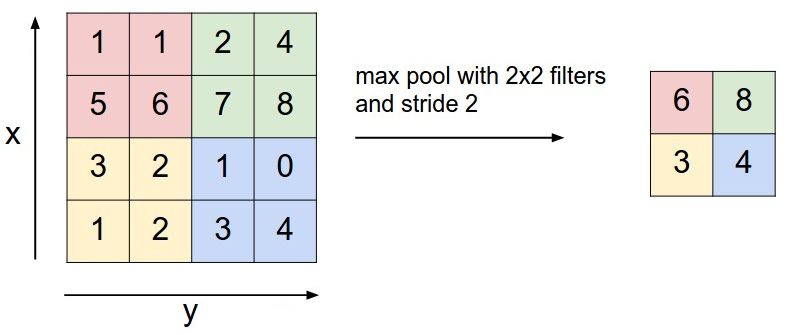
\includegraphics[scale=0.5]{img/max_pooling.jpeg}
        \caption[Illustration of a max pooling layer of stride 2]{Illustration of a max pooling layer of stride 2, i.e. it selects the maximum value from a $2 \times 2$ square}
        \label{fig:max_pooling}
    \end{figure}
    
    \item \textbf{Fully connected}: compute the class scores. As the name implied, this neuron is connected to all activations from the previous values. For classification, it corresponds to a loss function, a common one is the sigmoid:
    $$ \sigma (x) = \frac{1}{1 + \exp(-x)}$$
\end{itemize}

A CNN can also be used as a feature descriptor if we use the output of the last layers.
